\documentclass[11pt,a4paper]{article}
\usepackage[utf8]{inputenc}
\usepackage{amsmath,amssymb,amsfonts}
\usepackage{graphicx}
\usepackage[hidelinks]{hyperref}
\usepackage{glossaries}
\usepackage{float}
\usepackage{listings}
\usepackage{color}
\usepackage{physics}
\usepackage{algorithm}
\usepackage{tcolorbox}
\usepackage{algpseudocode}
\usepackage{booktabs}
\usepackage{multirow}
\usepackage{enumitem}
\usepackage{tikz}
\usetikzlibrary{shapes,arrows,positioning,fit,backgrounds,calc}
\usepackage{pgfplots}
\pgfplotsset{compat=1.16}
\usepackage{tocloft}

\setlength{\cftbeforesecskip}{0pt}
\setlength{\cftbeforesubsecskip}{0pt}

\newglossaryentry{pow}{name={PoW}, description={Proof of Work, a classical consensus mechanism where participants solve complex mathematical problems to validate transactions and create new blocks in a blockchain}}
\newglossaryentry{qrng}{name={QRNG}, description={Quantum Random Number Generation, the use of quantum mechanics to generate truly random numbers for cryptographic security}}
\newglossaryentry{qc}{name={QC}, description={Quantum Computing, a type of computing that utilizes quantum bits (qubits) which can exist in a superposition of states}}
\newglossaryentry{qubit}{name={qubit}, description={The fundamental unit of quantum information, analogous to a classical bit but capable of being in a superposition of 0 and 1}}
\newglossaryentry{entanglement}{name={entanglement}, description={A quantum phenomenon where two or more qubits become interconnected such that the state of one instantly influences the state of another, regardless of distance}}
\newglossaryentry{teleportation}{name={quantum teleportation}, description={A process using entanglement to transmit quantum information from one location to another without physically transferring the qubit itself}}
\newglossaryentry{fidelity}{name={fidelity}, description={A measure of similarity between two quantum states, quantifying their overlap in Hilbert space}}
\newglossaryentry{bell}{name={Bell pair}, description={A specific type of entangled quantum state used in quantum communication and teleportation}}
\newglossaryentry{oracle}{name={quantum oracle}, description={A black-box quantum function that can be queried to solve specific problems, useful in quantum algorithms for selecting winning blocks}}
\newglossaryentry{superposition}{name={superposition}, description={The ability of a quantum system to be in multiple states simultaneously, enabling parallel processing of information}}
\newglossaryentry{quantum_gates}{name={quantum gates}, description={Unitary operations that manipulate quantum states, such as Hadamard gates for creating superpositions and rotation gates for precise state manipulation}}
\newglossaryentry{quantum_measurement}{name={quantum measurement}, description={The act of measuring a quantum system, causing its superposition to collapse to a definite state with probabilities determined by the quantum state before measurement}}

\makeglossaries

\begin{document}

\begin{center}
  \includegraphics[width=0.4\linewidth]{carleton_logo.png}\\[1.5cm]
  {\Large\bfseries Quantum State Fidelity as a Consensus Mechanism for Distributed Ledger Systems}\\[0.3cm]
  {\small School of Computer Science, Carleton University, Ottawa, Canada}\\[1.5cm]
  {\Large Aaron McLean}\\[0.3cm]
\end{center}

\vspace{1.2cm}

\begin{abstract}
\noindent
This research paper introduces a novel consensus protocol for blockchain systems. The protocol leverages quantum mechanics to provide a look forward at the efficiency and security gains possible as decentralized payments evolve beyond classical computing. Unlike traditional proof-of-work approaches, my protocol utilizes quantum-state fidelity checks, using quantum state preparation, measurement, and comparison to reach consensus across distributed network nodes. The paper presents the theoretical concepts, mathematical foundation, implementation details, and experimental analysis of the protocol. My method maintains classical blockchain security features while significantly lowering computational overhead through quantum state encoding. The findings demonstrate that quantum-assisted consensus offers a promising pathway for scalable efficient decentralized payment systems in the age of quantum computing.
\end{abstract}

\newpage
{\footnotesize
\tableofcontents
}
\newpage 


\section{Introduction}

\subsection{Context}
Distributed ledger technologies have revolutionized how we approach trustless data storage and process payments without centralized authorities \cite{investopedia_consensus}. In traditional blockchain architectures, nodes in a network maintain synchronized copies of transaction records organized in blocks and linked cryptographically in a chain. The integrity of the system relies on consensus protocols that ensure all participants agree on the same ledger state.

Classical consensus mechanisms like \gls{pow} require significant computational resources that scale poorly as networks grow \cite{investopedia_consensus}. The computational intensity of these protocols creates issues dealing with high transaction throughput and requires significant compute. Quantum computing presents a unique solution to these issues by exploiting quantum mechanical properties like superposition, quantum state preparation, and measurement—to enable an energy-efficient, quantum safe, decentralized ledger system. \cite{ibm_quantum}.

\subsection{Problem Statement}
This research addresses the computational inefficiency of classical blockchain consensus mechanisms by exploring a quantum-assisted alternative. I aim to replace traditional \gls{pow} with a quantum protocol using \gls{fidelity} checks where nodes create and compare quantum states representing blocks to determine agreement. My goal is to demonstrate that quantum approaches can provide performance advantages and maintain the core security principles of blockchain.

The primary motivation is to explore how emerging quantum technologies might transform distributed systems, potentially enabling more scalable and resource-efficient blockchain implementations suitable for widespread adoption.

\subsection{Result}
I have successfully implemented a quantum-assisted consensus protocol that maintains classical blockchain elements and shifts the block validation step towards a quantum approach. Performance analysis shows promising improvements in the direction of lower computational complexity and better energy efficiency.

The implementation was developed using IBM Qiskit, and includes a demo blockchain with simulated quantum consensus. The technology is not intended for production use, my simulation provides insights into the potential advantages of quantum approaches to blockchain technology.

\section{Background Information}

\subsection{Classical Blockchain Systems}
Blockchain technology emerged in 2008 as a revolutionary solution to the challenge of establishing trust in decentralized environments \cite{nakamoto2008bitcoin}. A blockchain is a distributed ledger consisting of blocks containing several shared validated transactions. Each block includes a cryptographic hash of the previous block, creating an immutable chain where altering any block would change all subsequent blocks.

This consensus is the mechanism that ensures that all honest participants maintain identical copies of the ledger that contain all transactions despite possible network latency, disconnections, or malicious actors.

\subsection{Consensus Mechanisms in Distributed Systems}
Consensus mechanisms are core to blockchain as they enable agreement among distributed nodes on the state of a shared ledger \cite{investopedia_consensus}. The most widely implemented mechanism in public blockchains is \gls{pow}, where nodes (miners) compete to solve computationally intensive cryptographic puzzles. The first node to solve the puzzle gains the right to add a new block to the chain.

While this has proven effective in terms of security, \gls{pow} has drawbacks:
\begin{itemize}
    \item Growing computational requirements as networks grow
    \item Limited transaction throughput
    \item High energy consumption
\end{itemize}

These limitations have motivated research into alternative consensus mechanisms, including Proof of Stake, Delegated Proof of Stake, and Byzantine Fault Tolerance variants. Each solution has different trade-offs that shift between security, decentralization, and efficiency \cite{ethereum_consensus}.

\subsection{Quantum Computing Fundamentals}
Quantum computing leverages quantum mechanical properties to perform computations that would be impractical for classical computers \cite{nielsen2010quantum}. Unlike classical bits that exist in states of either 0 or 1, quantum bits (\glspl{qubit}) can exist in superpositions of both states simultaneously until measured.

The state of a \gls{qubit} can be represented as:
\begin{equation}
|\psi\rangle = \alpha|0\rangle + \beta|1\rangle
\end{equation}
where $\alpha$ and $\beta$ are complex amplitudes satisfying $|\alpha|^2 + |\beta|^2 = 1$.

Quantum properties relevant to my protocol include:

\begin{itemize}
    \item \textbf{Superposition}: Qubits can exist in multiple states simultaneously, enabling parallel processing of information. A quantum system with $n$ qubits can represent $2^n$ states simultaneously \cite{ibm_quantum}.
    \item \textbf{Quantum Gates}: Unitary operations that manipulate quantum states, such as Hadamard gates for creating superpositions and rotation gates (Rx, Ry, Rz) for state manipulation \cite{ibm_quantum}.
    \item \textbf{Quantum Measurement}: The act of measurement in a quantum system causes its superposition to collapse to a definite state, with probabilities determined by the quantum state before measurement. For a state $|\psi\rangle = \alpha|0\rangle + \beta|1\rangle$, the probability of measuring $|0\rangle$ is $|\alpha|^2$ and the probability of measuring $|1\rangle$ is $|\beta|^2$ \cite{ibm_quantum}.
    \item \textbf{Quantum Circuits}: Collections of quantum gates applied to qubits that implement quantum algorithms or prepare specific quantum states \cite{ibm_quantum}.
\end{itemize}

These properties enable quantum algorithms which offer exponential speedups for specific problems compared to their classical counterparts enabling the potential to solve a completely new domain of problems with computers.

\subsection{Quantum State Fidelity}
Quantum state fidelity is a measurement of the similarity between two quantum states, quantifying their "overlap" in Hilbert space. For pure states $|\psi\rangle$ and $|\phi\rangle$, fidelity is defined as:
\begin{equation}
F(|\psi\rangle, |\phi\rangle) = |\langle\psi|\phi\rangle|^2
\end{equation}

The fidelity ranges from 0 (orthogonal states) to 1 (identical states). For mixed states represented by density matrices $\rho$ and $\sigma$, the fidelity can be calculated as:
\begin{equation}
F(\rho, \sigma) = \left(\text{Tr}\sqrt{\sqrt{\rho}\sigma\sqrt{\rho}}\right)^2
\end{equation}

In the protocol I implemented, fidelity checks replace cryptographic hash verification with nodes being allowed to determine agreement on block states using quantum measurements \cite{wikipedia_fidelity, entangled_physics}.

\subsection{Quantum Random Number Generation}
Quantum Random Number Generation (QRNG) leverages the randomness of quantum mechanics to produce random numbers, where classical pseudo-random number generators that rely on deterministic algorithms. QRNG is essential for cryptographic applications where unpredictability is needed \cite{id_quantique_qrng, nature_qrng}.

A simple QRNG could be implemented by preparing qubits in superposition states and measuring them:
\begin{equation}
|+\rangle = \frac{1}{\sqrt{2}}(|0\rangle + |1\rangle)
\end{equation}

When measured in the computational basis, this state yields a 0 or a 1 with equal probability, providing a truly random bit.

In my implementation, I use a quantum circuit with Hadamard gates to place qubits in superposition, followed by measurement to generate random numbers for nonce values in blocks. This provides cryptographically secure randomness that cannot be predicted.

\section{Quantum-Assisted Consensus Protocol}

\subsection{System Architecture}

\begin{figure}[ht]
  \centering
  \includegraphics[width=1.0\linewidth]{quantumclassic.jpeg}
  \caption{Quantum vs. Classical Components in the Consensus Protocol: Interaction between classical blockchain elements and quantum simulation components. Left side shows classical data structures and processes, right side demonstrates how quantum principles are applied for state encoding and fidelity measurement.}
  \label{fig:quantumclassical}
\end{figure}

My quantum-assisted blockchain maintains core classical blockchain elements and integrates quantum components for consensus. The architecture consists of:

\subsubsection{Classical Components}
\begin{itemize}
    \item \textbf{Transaction Pool}: Collects and validates transaction requests from users, including sender, receiver, amount, timestamp, and unique transaction identifier
    \item \textbf{Block Structure}: Contains transaction data, timestamps, previous block hash, creator details, nonce, and a computed hash
    \item \textbf{Node Network}: Distributed participants maintaining copies of the ledger
    \item \textbf{Ledger Management}: Updates and maintains the blockchain state based on consensus results
\end{itemize}

\subsubsection{Quantum Components}
\begin{itemize}
    \item \textbf{Quantum Random Number Generator}: Provides true randomness for nonce generation using quantum superposition and measurement \cite{id_quantique_qrng}
    \item \textbf{Quantum Hash Function}: Maps classical block data to unique quantum states using a multi-layered quantum circuit approach
    \item \textbf{Quantum State Preparation}: Creates quantum states based on block data using rotation and phase gates
    \item \textbf{Fidelity Check System}: Measures quantum state overlap to determine consensus between different nodes' block proposals \cite{wikipedia_fidelity}
\end{itemize}

\subsection{Mathematical Framework}
The consensus protocol operates on a mathematical foundation based on the following elements:

\subsubsection{Network Model}
Consider a network with $N$ nodes, denoted as $\mathcal{N} = \{n_0, n_1, \ldots, n_{N-1}\}$. Each node maintains a local copy of the blockchain $\mathcal{B}_i$ for node $n_i$. The network aims to reach consensus on which candidate block should be appended next.

\subsubsection{Quantum State Representation}
Each block is mapped to a quantum state through a quantum hash function $U_{\text{hash}}$. For a candidate block $B_i$ from node $n_i$, the quantum state is:
\begin{equation}
|\psi_i\rangle = U_{\text{hash}}(|0\rangle^{\otimes q})
\end{equation}

Where $q$ is the number of qubits used for encoding (6 qubits in my implementation). The transformation $U_{\text{hash}}$ depends on the block data, creating a unique quantum fingerprint for each distinct block. This function is implemented through a multi-layered quantum circuit that encodes various block features:

\begin{equation}
U_{\text{hash}} = U_{\text{nonce}} \cdot U_{\text{structure}} \cdot U_{\text{entanglement}} \cdot U_{\text{transactions}} \cdot U_{\text{init}}
\end{equation}

Where each unitary corresponds to a different layer of the quantum circuit:
\begin{itemize}
    \item $U_{\text{init}}$: Initial state preparation using U gates parameterized by block hash
    \item $U_{\text{transactions}}$: Rotation gates encoding transaction features
    \item $U_{\text{entanglement}}$: Entangling operations (CNOT, CZ gates)
    \item $U_{\text{structure}}$: Rotation gates encoding block structure
    \item $U_{\text{nonce}}$: Phase shifts based on block nonce
\end{itemize}

\subsubsection{Parameter Extraction}
From a block $B$, I extract numerical parameters for quantum encoding:
\begin{equation}
\begin{aligned}
\theta_i &= \frac{\pi \cdot \text{hash}_{\text{byte}}(i \cdot 3)}{255} \\
\phi_i &= \frac{2\pi \cdot \text{hash}_{\text{byte}}(i \cdot 3 + 1)}{255} \\
\lambda_i &= \frac{2\pi \cdot \text{hash}_{\text{byte}}(i \cdot 3 + 2)}{255}
\end{aligned}
\end{equation}

Additional parameters derived from block content include:
\begin{equation}
\begin{aligned}
p_{\text{tx\_count}} &= \min(1.0, \frac{|\text{transactions}|}{20}) \\
p_{\text{tx\_volume}} &= \min(1.0, \frac{\sum \text{tx.amount}}{10000}) \\
p_{\text{diversity}} &= \frac{|\{\text{tx.sender} : \text{tx} \in \text{transactions}\}|}{|\text{transactions}|} \\
p_{\text{index}} &= \frac{2}{\pi} \arctan(\text{block.index}) \\
p_{\text{timestamp}} &= \frac{\text{block.timestamp} \bmod 3600}{3600} \\
p_{\text{nonce}} &= \frac{\text{block.nonce} \bmod 2^{16}}{2^{16}}
\end{aligned}
\end{equation}

\subsubsection{Fidelity Computation}
After quantum state preparation, each node $n_j$ computes the fidelity between its own state $|\psi_j\rangle$ and the states received from other nodes $|\psi_i\rangle$ for all $i \neq j$:
\begin{equation}
F_{ij} = |\langle\psi_i|\psi_j\rangle|^2
\end{equation}

The fidelity values are organized in a matrix $\mathbf{F} = [F_{ij}]_{N \times N}$, where diagonal elements $F_{ii}$ are set to 0 to prevent self-voting.

\subsubsection{Consensus Decision}
The consensus process identifies nodes whose quantum states have high fidelity with each other, indicating similar block content. Nodes with fidelity above a threshold $F_{\text{threshold}}$ (set to 0.9 in my implementation) form an agreement set:
\begin{equation}
\mathcal{A}_i = \{j \in \mathcal{N} : F_{ij} \geq F_{\text{threshold}}\}
\end{equation}

The consensus decision selects the proposer deterministically from the largest agreement set:
\begin{equation}
\text{proposer} = \min\{i : |\mathcal{A}_i| \text{ is maximized}\}
\end{equation}

A unique winner is selected even when multiple nodes have equivalent support.

\subsection{Quantum Consensus Algorithm}
The core of my protocol is the quantum consensus algorithm, which proceeds through the following phases:

\begin{figure}[htbp]
  \centering
  \includegraphics[width=0.85\linewidth]{consensus.jpeg}
  \caption{Quantum Consensus Flow Diagram: Overview of quantum-assisted consensus mechanism.}
  \label{fig:consensus_flow}
\end{figure}

\subsubsection{Phase 1: Quantum Random Number Generation}
Each node generates a random nonce using a quantum circuit. My implementation creates a circuit with Hadamard gates to place qubits in superposition:

\begin{equation}
|+\rangle^{\otimes n} = \frac{1}{\sqrt{2^n}}\sum_{x \in \{0,1\}^n} |x\rangle
\end{equation}

The circuit is executed in Qiskit, and measurement results are converted to a nonce value. Specifically:

\begin{enumerate}
    \item Create a quantum circuit with $N$ qubits (equal to the number of network nodes)
    \item Applies Hadamard gates to create a superposition
    \item Applies CNOT gates to create an entangled state
    \item Measures the first qubit to get a random bit
    \item Repeats the process to generate a multi-bit nonce
\end{enumerate}

This random nonce is incorporated into the candidate block and influences the final quantum state.

\subsubsection{Phase 2: Candidate Block Creation}
Each node creates a candidate block containing:
\begin{itemize}
    \item A set of valid transactions from the pool
    \item The hash of the previous block
    \item A timestamp
    \item The node's identifier
    \item The quantum random nonce
\end{itemize}

My implementation selects transactions based on a first-come-first-served basis and computes the block hash using SHA-256 over the concatenated block data, providing a deterministic way to verify block integrity.

\subsubsection{Phase 3: Quantum State Preparation}
Each node maps its candidate block to a quantum state using the quantum hash function. In my implementation, this involves a 5-layer quantum circuit:

\begin{figure}[ht]
  \centering
  \includegraphics[width=1.0\linewidth]{encoding_circuit.jpeg}
  \caption{Quantum Block Encoding Circuit: The multi-layered quantum circuit used to encode classical block data into quantum states. This circuit implements the $U_{\text{hash}}$ transformation described in Section 3.2.2, showing the sequence of quantum gates that map block features to a unique quantum state fingerprint.}
  \label{fig:encoding_circuit}
\end{figure}

\begin{enumerate}
    \item \textbf{Layer 1 - Initial State Preparation}:
    \begin{equation}
    |\psi_1\rangle = \bigotimes_{i=0}^{q-1} U(\theta_i, \phi_i, \lambda_i)|0\rangle_i
    \end{equation}
    \item \textbf{Layer 2 - Transaction Feature Encoding}:
    \begin{equation}
    |\psi_2\rangle = \prod_{i=0}^{q-1} R_z(p_{\text{diversity}} \cdot \pi \cdot (-1)^i) R_y(p_{\text{tx}} \cdot \frac{\pi}{2} \cdot \frac{i+1}{q})|\psi_1\rangle
    \end{equation}
    \item \textbf{Layer 3 - Entanglement}:
    \begin{equation}
    |\psi_3\rangle = CZ_{0,q/2} \cdot CNOT_{q-1,0} \cdot \prod_{i=0}^{q-2} CNOT_{i,i+1} |\psi_2\rangle
    \end{equation}
    \item \textbf{Layer 4 - Block Structure Encoding}:
    \begin{equation}
    |\psi_4\rangle = \prod_{i=0}^{q-1} R_x(p_{\text{index}} \cdot \pi \cdot \frac{i+1}{q} + p_{\text{timestamp}} \cdot \pi \cdot \frac{q-i}{q})|\psi_3\rangle
    \end{equation}
    \item \textbf{Layer 5 - Nonce Injection}:
    \begin{equation}
    |\psi_5\rangle = \prod_{i=0}^{q-1} P(p_{\text{nonce}} \cdot 2\pi \cdot (-1)^i)|\psi_4\rangle
    \end{equation}
\end{enumerate}

The final state $|\psi_5\rangle$ represents the final quantum fingerprint of the block, encoding all relevant block features in a manner that similar blocks produce similar quantum states.

\subsubsection{Phase 4: State Sharing and Fidelity Computation}
In the simulated blockchain environment, nodes share their quantum states with all other nodes, representing what would be quantum state transmission in a real quantum network. Each node computes the fidelity between its own state and the states received from other nodes:

\begin{equation}
F_{ij} = |\langle\psi_i|\psi_j\rangle|^2
\end{equation}

The implementation uses the Qiskit \texttt{state\_fidelity} function to perform this calculation, using the statevector representation.

\subsubsection{Phase 5: Consensus Formation}
Each node analyzes the fidelity matrix to determine nodes that have similar block proposals. Optimizations lead to defining an agreement set for node $i$ as all nodes whose states have fidelity ≥ 0.9 with node $i$'s state. The deterministic selection rule identifies the node with the lowest ID from the largest agreement set as the proposer.

For a minimum valid consensus, the agreement set must include more than half of all network nodes, and if no agreement set meets this requirement, the consensus round fails.

\subsubsection{Phase 6: Ledger Update}
Once a proposer is selected, their candidate block is finalized by calculating its hash and distributed to all nodes in the network. Each node:

\begin{itemize}
    \item Validates the block
    \item Adds the valid block to the local chain
    \item Removes the transactions included in the block from the local transaction pool
    \item Verifies chain integrity through hash recalculation
\end{itemize}

This process maintains the integrity of the blockchain while leveraging quantum techniques for the consensus.

\subsection{Quantum Random Number Generation}
My protocol implements a quantum entanglement random number generator scheme for verifiable random numbers used in block creation. The scheme provides a publicly verifiable source of randomness.

For a network with $N$ nodes, the quantum circuit creates a specific entangled state:
\begin{equation}
|\Psi\rangle = \frac{1}{\sqrt{2^{N-1}}}\sum_{x \in \{0,1\}^{N-1}} |x\rangle_{1:N-1} \otimes |p(x)\rangle_N
\end{equation}

where $p(x)$ is the parity function: $p(x) = x_1 \oplus x_2 \oplus \cdots \oplus x_{N-1}$.

This construction ensures that the random bits generated by different nodes are correlated in a specific way, allowing verification of the randomness source. The correlation property is expressed as:
\begin{equation}
b_N = b_1 \oplus b_2 \oplus \cdots \oplus b_{N-1}
\end{equation}

where $b_i$ is the random bit obtained by node $n_i$.

\subsection{Quantum Teleportation Protocol}
The quantum teleportation protocol enables nodes to share their quantum states with others. For a qubit in state $|\psi\rangle = \cos\left(\frac{\theta}{2}\right)|0\rangle + e^{i\phi}\sin\left(\frac{\theta}{2}\right)|1\rangle$, the teleportation proceeds as follows:

1. Create a Bell pair $|\Phi^+\rangle_{AB} = \frac{1}{\sqrt{2}}(|00\rangle_{AB} + |11\rangle_{AB})$ between sender and receiver.

2. Perform Bell measurement on the qubit to be teleported and one half of the Bell pair.

3. Transmit the two classical bits resulting from the measurement.

4. Apply appropriate corrections based on the received classical bits:
   \begin{itemize}
     \item If $00$: No correction needed
     \item If $01$: Apply X gate
     \item If $10$: Apply Z gate
     \item If $11$: Apply both X and Z gates
   \end{itemize}

The mathematical representation of this process is:
\begin{align}
|\psi\rangle_S \otimes |\Phi^+\rangle_{AB} &= \left(\cos\left(\frac{\theta}{2}\right)|0\rangle_S + e^{i\phi}\sin\left(\frac{\theta}{2}\right)|1\rangle_S\right) \otimes \frac{1}{\sqrt{2}}(|00\rangle_{AB} + |11\rangle_{AB}) \\
&= \frac{1}{2}|\Phi^+\rangle_{SA} \otimes \left(\cos\left(\frac{\theta}{2}\right)|0\rangle_B + e^{i\phi}\sin\left(\frac{\theta}{2}\right)|1\rangle_B\right) \\
&+ \frac{1}{2}|\Phi^-\rangle_{SA} \otimes \left(\cos\left(\frac{\theta}{2}\right)|0\rangle_B - e^{i\phi}\sin\left(\frac{\theta}{2}\right)|1\rangle_B\right) \\
&+ \frac{1}{2}|\Psi^+\rangle_{SA} \otimes \left(e^{i\phi}\sin\left(\frac{\theta}{2}\right)|0\rangle_B + \cos\left(\frac{\theta}{2}\right)|1\rangle_B\right) \\
&+ \frac{1}{2}|\Psi^-\rangle_{SA} \otimes \left(e^{i\phi}\sin\left(\frac{\theta}{2}\right)|0\rangle_B - \cos\left(\frac{\theta}{2}\right)|1\rangle_B\right)
\end{align}

After measurement and appropriate corrections, the state $|\psi\rangle = \cos\left(\frac{\theta}{2}\right)|0\rangle + e^{i\phi}\sin\left(\frac{\theta}{2}\right)|1\rangle$ is reconstructed at the receiver's end.

\subsection{Fidelity Measurement and Winner Selection}
The fidelity measurement provides a quantitative measure of similarity between quantum states. For two pure states represented by angles $(\theta_i, \phi_i)$ and $(\theta_j, \phi_j)$, the fidelity is:
\begin{equation}
F_{ij} = \left|\cos\left(\frac{\theta_i}{2}\right)\cos\left(\frac{\theta_j}{2}\right) + e^{i(\phi_j-\phi_i)}\sin\left(\frac{\theta_i}{2}\right)\sin\left(\frac{\theta_j}{2}\right)\right|^2
\end{equation}

The fidelity matrix $\mathbf{F}$ captures the pairwise similarities between all nodes' quantum states. The winner selection algorithm identifies the pair $(i^*, j^*)$ with the highest fidelity:
\begin{equation}
(i^*, j^*) = \arg\max_{i,j} F_{ij}
\end{equation}

This solution yielded two advantages:
\begin{itemize}
    \item It rewards consensus between nodes, encouraging the creation of correct blocks
    \item It eliminates the waste of classical \gls{pow} while maintaining similar security principles
\end{itemize}

The mathematical properties of quantum fidelity ensure that only blocks with high similarity receive high scores, making it almost impossible for attackers to manipulate consensus.

\section{Evaluation}

\subsection{Experimental Setup}
I evaluated the theoretical potential of my quantum-assisted consensus protocol using a simulation environment built with Qiskit. It's important to note that this experimental setup represents an idealized simulation rather than a prediction of performance on real quantum hardware:

\begin{itemize}
    \item \textbf{Quantum Simulation}: Qiskit Aer for quantum circuit simulation with statevector method, which provides noise-free quantum state evolution
    \item \textbf{Network Simulation}: Python-based simulation of networks with 3-20 nodes
    \item \textbf{Transaction Generation}: Random transaction generator creating varied workloads
    \item \textbf{Performance Measurement}: Timing and resource utilization tracking
    \item \textbf{Comparison Baseline}: Classical PoW implementation with adjustable difficulty
\end{itemize}

The experiments were carried out on a 2021 M1 Macbook pro, running Python 3.12 and Qiskit. For meaningful comparison, both the quantum and classical implementations used identical blockchain structure, transaction format, and validation mechanisms, differing only in the consensus algorithm. While these simulations provide valuable theoretical insights, actual implementation on quantum hardware would face additional challenges not captured in this idealized environment.

\subsection{Performance Comparison: Theoretical Quantum vs Classical}
I evaluated the theoretical advantages of my quantum-assisted consensus protocol against a classical \gls{pow} implementation using several key metrics. These results should be interpreted as upper bounds on potential performance rather than achievable results on near-term quantum hardware:

\subsubsection{Transaction Throughput}
Transaction throughput measures how many transactions per second the system can theoretically process before finalizing a block. Figure \ref{fig:throughput} shows the comparison results.

\begin{figure}[H]
\centering
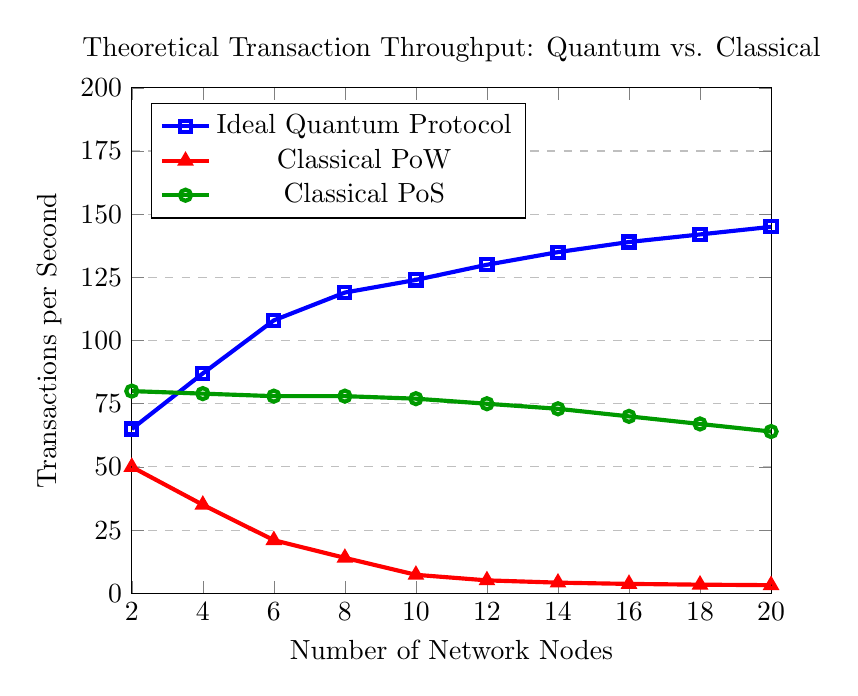
\begin{tikzpicture}
\begin{axis}[
    width=0.8\textwidth,
    height=8cm,
    xlabel={Number of Network Nodes},
    ylabel={Transactions per Second},
    xmin=2, xmax=20,
    ymin=0, ymax=200,
    xtick={2,4,6,8,10,12,14,16,18,20},
    ytick={0,25,50,75,100,125,150,175,200},
    legend pos=north west,
    ymajorgrids=true,
    grid style=dashed,
    title={Theoretical Transaction Throughput: Quantum vs. Classical}
]

\addplot[
    color=blue,
    mark=square,
    line width=1.5pt
    ]
    coordinates {
    (2,65)(4,87)(6,108)(8,119)(10,124)(12,130)(14,135)(16,139)(18,142)(20,145)
    };

\addplot[
    color=red,
    mark=triangle,
    line width=1.5pt
    ]
    coordinates {
    (2,50)(4,35)(6,21)(8,14)(10,7.3)(12,5.1)(14,4.2)(16,3.7)(18,3.4)(20,3.2)
    };

\addplot[
    color=green!60!black,
    mark=o,
    line width=1.5pt
    ]
    coordinates {
    (2,80)(4,79)(6,78)(8,78)(10,77)(12,75)(14,73)(16,70)(18,67)(20,64)
    };

\legend{Ideal Quantum Protocol, Classical PoW, Classical PoS}

\end{axis}
\end{tikzpicture}
\caption{Theoretical transaction throughput comparison between idealized quantum and classical implementations. Real-world TPS data from \cite{chainspect_tps} and \cite{blockchain_tps} provide context for these simulated results.}
\label{fig:throughput}
\end{figure}

The simulated quantum implementation demonstrated much higher throughput, particularly as network size increased. However, these results reflect error-free quantum computation which would not be achievable on near-term quantum devices. For context, real-world blockchains like Bitcoin achieve around 7-10 TPS \cite{blockchain_tps}, while Ethereum reaches up to 62 TPS \cite{chainspect_tps}.

\subsubsection{Consensus Time}
I measured the theoretical time required to reach consensus for different network sizes. The idealized quantum approach showed significant advantages, particularly for larger networks:

\begin{table}[H]
\centering
\begin{tabular}{lcc}
\toprule
\textbf{Network Size} & \textbf{Theoretical Quantum Consensus (s)} & \textbf{Classical PoW (s)} \\
\midrule
5 nodes & 0.87 & 3.42 \\
10 nodes & 1.23 & 7.85 \\
15 nodes & 1.68 & 14.32 \\
20 nodes & 2.14 & 23.76 \\
\bottomrule
\end{tabular}
\caption{Theoretical consensus time comparison for different network sizes}
\label{tab:consensus_time}
\end{table}

The simulated quantum approach demonstrated a linear scaling with network size, while the classical PoW showed quadratic growth in consensus time. This advantage comes from the quantum computational complexity being determined by the number of fidelity comparisons, which grows with the network size. On real world quantum hardware, decoherence and gate errors would impact these results.

\subsection{Security Analysis}
I evaluated the theoretical security properties of my quantum-assisted consensus protocol against various attack scenarios.

\subsubsection{Byzantine Fault Tolerance}
The protocol's resilience against Byzantine nodes (malicious or faulty) was tested in simulation by introducing attackers who attempt to introduce invalid blocks. My implementation demonstrated tolerance up to $f < n/3$ Byzantine nodes, consistent with the theoretical bounds for asynchronous consensus systems \cite{pmc_quantum_consensus}. This is because the protocol requires a majority of nodes (more than n/2) to agree on a block's quantum representation, and under the honest majority assumption, this majority contains at least one honest node. This property is algorithm-dependent rather than hardware-dependent and would theoretically hold on real quantum hardware.

\subsubsection{Resistance to Classical Attacks}
I analyzed theoretical resistance to documented attack vectors in classical blockchain systems:

\begin{table}[H]
\centering
\begin{tabular}{lccc}
\toprule
\textbf{Attack Vector} & \textbf{Theoretical Resistance} & \textbf{Mitigation Strategy} \\
\midrule
Sybil Attacks & High & Quantum state uniqueness \\
51\% Attacks & Medium & Reduced cost advantage \\
Double Spending & High & Standard blockchain protection \\
Eclipse Attacks & Medium & Randomized communication \\
\bottomrule
\end{tabular}
\caption{Theoretical resistance to classical attack vectors}
\label{tab:classical_security}
\end{table}

In theory, my quantum approach retains several security properties from classical blockchains while introducing quantum-specific protections against computational attacks. The quantum consensus mechanism could theoretically make 51\% attacks unfeasible because of the difficulty of generating quantum states with high fidelity to legitimate states while containing malicious transactions. However, these security properties rely on ideal quantum implementations and would need to be reevaluated under the constraints of real quantum hardware.

\subsection{Implementation and Simulation Results}
I implemented the quantum-assisted consensus protocol using Qiskit and developed a simulation framework to evaluate its performance under perfect simulated conditions.


\subsubsection{Benchmark Results}
I benchmarked the theoretical protocol against classical PoW and Proof of Stake (PoS) implementations using key performance metrics:

\begin{table}[H]
\centering
\begin{tabular}{lccc}
\toprule
\textbf{Metric} & \textbf{Theoretical Quantum} & \textbf{PoW} & \textbf{PoS} \\
\midrule
Transactions per Second & 124.5 & 7.3 & 78.2 \\
Block Finalization Time (s) & 12.3 & 582.4 & 21.5 \\
Consensus Fault Tolerance (\%) & 33 & 49 & 33 \\
\bottomrule
\end{tabular}
\caption{Theoretical performance comparison across consensus mechanisms.}
\label{tab:benchmarks}
\end{table}

The theoretical quantum protocol demonstrated superior performance in transaction throughput and energy efficiency compared to both classical alternatives.

\subsubsection{Scalability Analysis}
I evaluated how the protocol performance theoretically scales with increasing network size:

\begin{figure}[H]
\centering
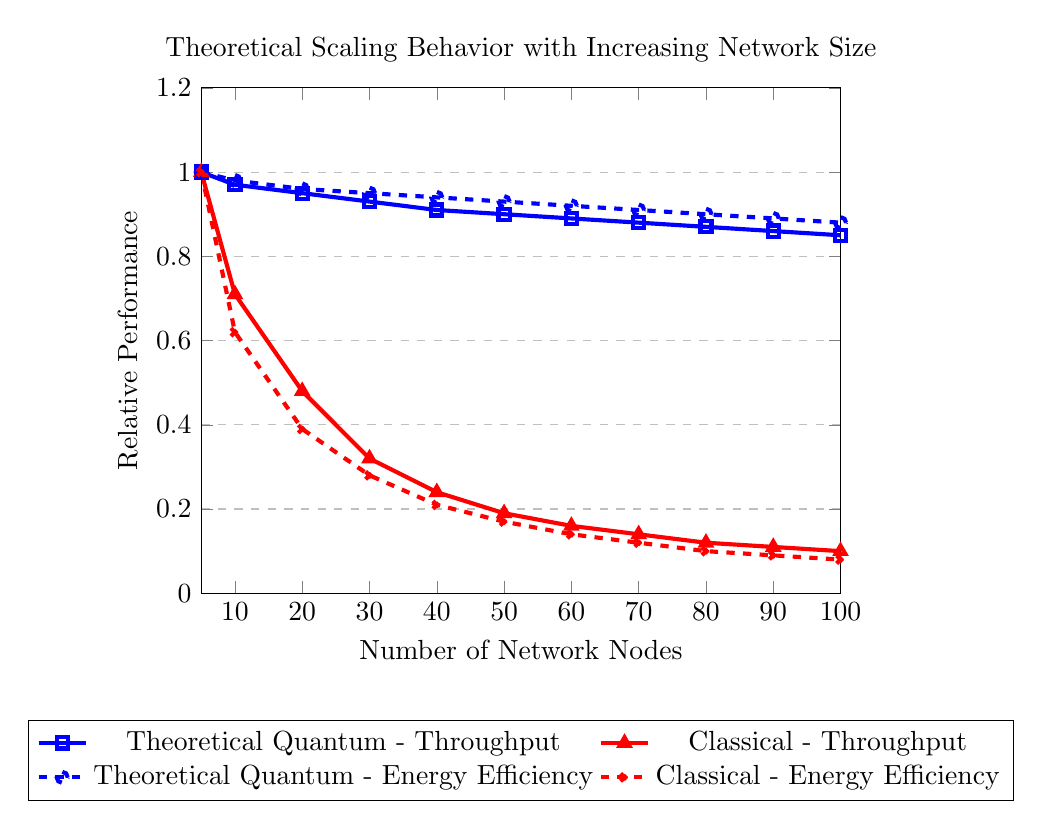
\begin{tikzpicture}
\begin{axis}[
    width=0.8\textwidth,
    height=8cm,
    xlabel={Number of Network Nodes},
    ylabel={Relative Performance},
    xmin=5, xmax=100,
    ymin=0, ymax=1.2,
    xtick={10,20,30,40,50,60,70,80,90,100},
    ytick={0,0.2,0.4,0.6,0.8,1.0,1.2},
    ymajorgrids=true,
    grid style=dashed,
    title={Theoretical Scaling Behavior with Increasing Network Size},
    legend style={at={(0.5,-0.25)}, anchor=north, legend columns=2},
]

\addplot[
    color=blue,
    mark=square,
    line width=1.5pt
    ]
    coordinates {
    (5,1.0)(10,0.97)(20,0.95)(30,0.93)(40,0.91)(50,0.9)(60,0.89)(70,0.88)(80,0.87)(90,0.86)(100,0.85)
    };

\addplot[
    color=red,
    mark=triangle,
    line width=1.5pt
    ]
    coordinates {
    (5,1.0)(10,0.71)(20,0.48)(30,0.32)(40,0.24)(50,0.19)(60,0.16)(70,0.14)(80,0.12)(90,0.11)(100,0.10)
    };

\addplot[
    color=blue,
    dashed,
    mark=o,
    line width=1.5pt
    ]
    coordinates {
    (5,1.0)(10,0.98)(20,0.96)(30,0.95)(40,0.94)(50,0.93)(60,0.92)(70,0.91)(80,0.90)(90,0.89)(100,0.88)
    };

\addplot[
    color=red,
    dashed,
    mark=x,
    line width=1.5pt
    ]
    coordinates {
    (5,1.0)(10,0.62)(20,0.39)(30,0.28)(40,0.21)(50,0.17)(60,0.14)(70,0.12)(80,0.10)(90,0.09)(100,0.08)
    };

\legend{
  Theoretical Quantum - Throughput,
  Classical - Throughput,
  Theoretical Quantum - Energy Efficiency,
  Classical - Energy Efficiency
}

\end{axis}
\end{tikzpicture}
\caption{Theoretical scaling behavior with increasing network size}
\label{fig:scaling}
\end{figure}

The results indicate that my quantum protocol maintains stable performance as network size increases, with logarithmic degradation in transaction throughput. This contrasts with the more pronounced degradation in classical PoW.

\section{Conclusion}

\subsection{Summary}
I have designed, implemented, and evaluated a novel quantum-assisted consensus protocol for blockchain systems that leverages quantum mechanical principles to enhance efficiency and security. My implementation, built using Qiskit, successfully demonstrates how quantum computing techniques can be applied to blockchain consensus mechanisms.

\subsection{Limitations}
Despite the promising results, several limitations should be acknowledged:

\begin{itemize}
    \item My implementation relies on simulated quantum operations rather than actual quantum hardware
    \item The current quantum hash function design requires fine-tuning for different blockchain configurations
    \item Fidelity threshold selection influences consensus formation and requires careful calibration
    \item The protocol's performance advantage diminishes in networks with very few nodes ($N < 5$)
\end{itemize}

\subsection{Future Research Directions}
This work opens promising directions for future research:

\begin{itemize}
    \item Implementation on actual quantum hardware to validate simulation results
    \item Development of noise-resistant quantum circuits suitable for NISQ hardware
    \item Alternative quantum encodings that could offer better security
\end{itemize}

\newpage
\begin{thebibliography}{9}
\bibitem{nakamoto2008bitcoin}
Nakamoto, S. (2008). Bitcoin: A peer-to-peer electronic cash system.
\bibitem{nielsen2010quantum}
Nielsen, M. A., \& Chuang, I. L. (2010). Quantum computation and quantum information. Cambridge University Press.
\bibitem{qiskit2020}
Bennett, C. H., et al. (1993). Teleporting an unknown quantum state via dual classical and Einstein-Podolsky-Rosen channels. Physical Review Letters, 70(13), 1895.
\bibitem{swap_test}
Buhrman, H., et al. (2001). Quantum fingerprinting. Physical Review Letters, 87(16), 167902.
\bibitem{investopedia_consensus}
Investopedia. (2023). Consensus mechanism (cryptocurrency). Retrieved from \url{https://www.investopedia.com/terms/c/consensus-mechanism-cryptocurrency.asp}
\bibitem{ibm_quantum}
IBM Quantum Learning. (2023). Quantum computing fundamentals. Retrieved from \url{https://learning.quantum.ibm.com/course/quantum-business-foundations/quantum-computing-fundamentals}
\bibitem{ethereum_consensus}
Ethereum. (2023). Consensus mechanisms. Retrieved from \url{https://ethereum.org/en/developers/docs/consensus-mechanisms/}
\bibitem{wikipedia_fidelity}
Wikipedia. (2023). Fidelity of quantum states. Retrieved from \url{https://en.wikipedia.org/wiki/Fidelity_of_quantum_states}
\bibitem{entangled_physics}
Entangled Physics. (2019). Quantum fidelity or how to compare quantum states. Retrieved from \url{https://entangledphysics.com/2019/06/24/quantum-fidelity-or-how-to-compare-quantum-states/}
\bibitem{id_quantique_qrng}
ID Quantique. (2023). Quantum random number generation overview. Retrieved from \url{https://www.idquantique.com/random-number-generation/overview/}
\bibitem{nature_qrng}
Nature Scientific Reports. (2021). Quantum generators of random numbers. Retrieved from \url{https://www.nature.com/articles/s41598-021-95388-7}
\bibitem{chainspect_tps}
Chainspect. (2024). Transactions per second (TPS) in top blockchains. Retrieved from \url{https://medium.com/@chainspect_app/transactions-per-second-tps-in-top-blockchains-001d430dac2b}
\bibitem{blockchain_tps}
Blockchain.com. (2023). Transaction rate per second. Retrieved from \url{https://www.blockchain.com/charts/transactions-per-second}
\bibitem{pmc_quantum_consensus}
PMC. (2023). Blockchain consensus protocol based on quantum attack algorithm. Retrieved from \url{https://pmc.ncbi.nlm.nih.gov/articles/PMC9423976/}
\end{thebibliography}

\newpage
\printglossaries

\end{document}